
%\begin{itemize}
%    \item do we need any hard numbers beyond per-event size of %PHYS(LITE)? Target Event Processing Rate? 
%    PHYS: 50kb/event (currently 38 kb/event but missing some trigger %info and maybe other stuff)
%    PHYSLITE: 10 kb/event
%\end{itemize}

%Probably need to condense, for me main points for R4 are

%\begin{itemize}
%\item PHYS/PHYSLITE
%\item Integration into wider data science 
%\item Data Access 
%\item Interactive Analysis at HL-LHC scale
%\item (Analysis Automation)
%\end{itemize}

%Open Q:
%\begin{itemize}
%\item what about DAST/WLCG obv will evolve do we discuss it? AL: not %sure we should
%\item epxect accelerators  to be useful (e.g. github/hepaccelerate) AL: %Yes but can we say anything other than this?
%\end{itemize}

\subsection{Introduction}

While the vast majority computational resources at the LHC are spent on preparing reconstructed data and simulation datasets, a large fraction of human resources is spent on the analysis of the data collected by the experiment to produce physics results. It is imperative that the Analysis Model is conducive to a streamlined workflow which is easily usable to a typical analyst, with particular focus on enabling easy access to students at all levels. 
In light of the data volumes expected at the HL-LHC, an evolution of the current data reduction workflow~\cite{Derivation System} that consolidates the generation of  calibrated event data for analysis is important. In the baseline analysis model, the HL-LHC sees the full deployment and adoption of of the new data formats introduced during Run 3. In addition, on the timescale of the HL-LHC, the tool-chest accessible to physicists will broaden as industry tools for large scale data analysis develop and are incorporated into the HEP ecosystem. The analysis model must therefore serve both traditional and modern analysis tools. While these are not 'baseline', the early adoption of industry-standard tools should be encouraged and should replace traditional tools during Run 4.

\subsection{Analysis Data Formats}


A core recommendation of the AMSG-3 Task Force\cite{amsg3} is the introduction of two new common, data formats, {\sc DAOD\_PHYS} ($\sim$ 50kb/event) and {\sc DAOD\_PHYSLITE} ($\sim$ 10 kb/event). 
While Run 2's introduction of a centralized data reduction format (the Derivation Framework) was successful, a significant overlap in the derivations defined across the various analysis groups is observed. This motivated the common {\sc DAOD\_PHYS} format as a way to reduce disk space usage. This format is designed to include sufficient event data to perform final object calibration, though those object calibrations will not yet be applied.
On the other hand, the light-weight {\sc DAOD\_PHYSLITE} format will be a centrally produced data format for events in which all 'object' calibrations are already applied. To that end, the `CP Algorithms' maintained by the Analysis Model Group and the performance group, provide standard building blocks.
The goal of these data formats is to cover the needs of 'most' (~80\%?) ATLAS data analyses.
The remaining analyses will be served using custom derivations and (DRAW) filters with every effort made to reduce the number of processed events.

In the current computing model, a large amount of disk space, and significant human time, is typically taken up by processing and storing systematic variations on the calibrated objects.
In order to access systematic variations in the {\sc DAOD\_PHYSLITE} event data it will be required that these can be retrieved using standard interfaces based on e.g. particle object interfaces.




\subsubsection{Storage needs}
% 50 kb/event for PHYS, 10 kb/evnt PHYSLITE
% 2 trillion events (take latest from Johannes) 2 PB/year PHYSLITE 0.5 PB

Assuming $2 \times 10^{11}$\;($5\times 10^{10}$) events per year for simulation (data) at the AOD level the expected size at {\sc DAOD\_PHYS} will 100PB\;(12 PB) per year of {\sc PHYS} data, while at {\sc DAOD\_PHYSLITE} 2PB (0.5 PB) per year are projected. As the vast majority of analyses are expected to use these formats, the AODs (200 PB (35 PB) per year) need not be available on hot storage but rather served from tape using a data carousal approach (cite?). Additionally, it is foreseen that {\sc PHYSLITE} can be derived from the already-reduced {\sc PHYS} format instead of from {\sc AOD}, which will only need to be then accessed when calibration algorithms and recommendations are renewed. of the latter An option being pursued is that it may be feasible to forgo persistent storage of AODs for most data streams and rather rely on the ability to re-generate AODs on-demand. A similar strategy was successfully pursued for the Event Summary Data (ESD) format before the second data-taking run of ATLAS.

% this is now the 'wish list' part

\subsubsection{Potential future improvements}
The {\sc PHYSLITE} format should enable columnar data access and enable the collaboration to provide analyzers with a common event data model (EDM) on which analysis tools can rely. The xAOD model of jagged data containers and light-weight ``interface EDM classes'' has been not only applied within the context of ATLAS but similar patterns are emerging in new HEP data analysis tools.  Columnar data may be served to the analyzer either over the network or from on-disk columnar data formats such as ROOT, Parquet, etc.

\subsection{Running on the Data}
% Should the new RNtuple be mentioned here?
% Life without an AOD
% Life without AnalysisBase or AthAnalysis?

There are three paths analyzer can take from the derived data  to plots and tables of numbers. The path will depend on the type of data the physics analysis needs:
\begin{enumerate}
    \item PHYSLITE - This format will be easily readable without a collaboration-specific framework. A light-weight event data model library will using common tools will be provided to aid in its use. For example, this library will make it easy to derive systematic variations. Development work is required to get to baseline usage.
    \item PHYS - This format is xAOD ROOT based, much like the current xAOD's used by ATLAS in Run 2. In that sense, the tools and frameworks are already currently available. CP Tools, which apply the object calibrations should continue to be maintained as they are for Run 2. Further those CP tools will be used in the production of PHYSLITE.
    \item DRAW/Derivations - Unfortunately a small number of analyses will not be able to use either the PHYS or PHYSLITE format (long-lived particle searches are an example). The workflow for these analyses will look very similar to how it looks now: a derivation will be run, and analyzers will run on the results of that derivation. 
\end{enumerate}

ATLAS will be expected to supply the resources to run on these centrally produced datasets. The model for DRAW/Derivations is exactly as it is now: the physics analyzer will likely submit a GRID job to process the {\tt rucio} dataset containers and then download the resulting datasets locally. These are expensive jobs as calibrations have to be applied and systematic errors derived - which frequently takes about 1 second per event. The PHYS dataset will be approximately 12 PB/year of HL-LHC running. For datasets this size it will not be possible to submit jobs ad-hoc - instead the experiment's Derivation Framework will have to be used. Full runs will be restricted to twice a year (and likely at the same time as the production of PHYSLITE). This will require adaptation by physics groups who have written their own frameworks in Run 2. PHYSLITE, at about 0.5 PB/year, is small enough not to require any special approach to run. It is assumed physicists will submit jobs on the GRID as required to run against PHYSLITE. The experiment will need to maintain enough copies of PHYSLITE to support quick and efficient access. If this is not the case, analyzers will likely start to create and try to save new derivations, nullifying the potential disk space savings.

%A consequence of the adoption of fewer types of derivation formats will be the reduced need for different analysis frameworks. Run-2 saw a consolidation of data analysis frameworks around two base approaches, one based on standalone {\sc ROOT} (AnalysisBase) and another based on {\sc Athena} (AthAnalysis), but a large number of group-specific frameworks derived from these two approaches remain.

%Broadly speaking analysis frameworks currently do two things. First, they apply the final object calibration (and associated systematic uncertainties). Secondly, they carry out analysis selection (often looser than needed for the final interpretation) and data augmentation (e.g. computing of new variables). Thus the broad adoption of {\sc DAOD\_PHYSLITE} will enable much lighter-weight analysis frameworks that can focus only on the second task, reducing not only the complexity of the code but the resources needed to process the events.

%The further simplification for {\sc PHYSLITE} based frameworks should facilitate further reduction in the number and complexity of the frameworks maintained by the physics groups as well as possibly a single base analysis framework. 
% THIS IS WHERE ALISON GOT TO!!!

A crucial element of analyses is the interpretation of results using suitable statistics software. In Run-2 this often required format conversions to standalone Ntuple-data, as this software is developed independently from the xAOD format, often incurring significant storage cost in analysis teams. Minimizing the overhead of using a light-weight event data model with {\sc PHYSLITE} and enabling its `framework-less' processing should reduce the need for such format transformations.

\subsubsection{Potential future improvements}

Techniques outlined above are the traditional analysis techniques used by ATLAS in Run 2. There are several developments in the HEP software ecosystem that could improve the efficiency with which we access and reduce the data: ROOT's RDataFrame and RNTuple, tools from the python ecosystem, and distributed analyses and modern high-performance distributed tools. Finally there is also the tantilizing idea of using co-processors to speed up analysis (e.g. GPU's or FPGA's).

\paragraph{RDataFrame and RNTuple}

As ROOT7 moves towards release, two big projects are of potential interest to ATLAS analyzers: RDataFrame and RNTuple. RDataFrame is a declarative analysis tool optimized to process large amounts of ROOT data with a fairly simple API. It supports, out of the box, multi-threaded, simple selection semantics, along with virtual columns and other features commonly needed during data reduction. We expect RDataFrame to be one of the primary way people who want to remain in the ROOT environment to run on PHYSLITE. Development work by ATLAS must be done to make sure that the PHYSLITE libraries can be used in the RDataFrame multi-threaded environment. ATLAS should also track Analysis Facilities developments based on RDataFrame.

RNTuple is a new high speed data format - the next generation TTree/TFile. The ROOT Team is currently finalizing the RNTuple work. This is a potential new file format for PHYSLITE and ATLAS should allocate time to investigate its performance characteristics like speed, storage space, etc.

\paragraph{The Python Ecosystem as an Analysis Platform}

In the wider domain of data intensive physical sciences and Machine Learning, the use of the Python programming language as the primary entry point for data analaysis has increased significantly and a collection of tools, commonly referred to as the `scientific Python ecosystem', has emerged. The core packages of this ecosystem are numerical libraries for vectorized array computation, NumPy\cite{numpy}, algorithms (SciPy \cite{scipy}), Visualization (Matplotlib \cite{matplotlib} ) and others. While ROOT provided data analysts with many of these functionalities, it is desirable for the ATLAS data analysis model to provide avenues through which a seamless integration of the tools provided by the ecosystem as data analysts can rely on a broad community beyond the confines of HEP. An integration will also enable the collaboration to capitalize on distributed computing for data analysis developed outside of HEP. An important connecting component here is the {\tt uproot}\cite{uproot-library} library, which provides read and write capabilities for the ROOT format.

In the context of the HEP Software Foundation, the development of HEP-specific applications 

increasing effort on PyHEP ecosystem, event-level processing (example: coffea) , statistics (examples: zfit, pyhf), easy integration with wider data science toolset. 
Can we integrate ATLAS EDM seamlessly (read xAOD in uproot?), or rather extract columns w   ServiceX and go from there? (you'll have ServiceX regardless, and if you get this stuff working with uproot you'll want to put it into ServiceX too).

\paragraph{Fast Serving of Data to the Analyzer}

% Double check other mentions of idds in the document and make sure we are in line with its usage!

Data storage in the HL-LHC era is evolving towards a Data Lake managed by {\tt rucio}. To improve access tools that do basic transforms near the data are being implemented in the forms of the iDDS~\cite{idds} and ServiceX~\cite{servicex} projects. The tools, working together, with high bandwidth access to the data can skim and apply basic transformations. For example, the analyzer can request all events with 2 clean jets and jet $p_T>300$ GeV, and have it delivered in close to real time. The nominal access pattern for this sort of data is to submit a GRID Job: this will run on a dedicated cluster optimized to access the data and deliver only what is needed. Output formats include ROOT based files as well as columnar data (in the arrow format, for example). Groups in ATLAS are working on these tools, and support from ATLAS will be required if they are to be integrated into Operations.

\paragraph{Distributed interactive analysis, out-of-core Data Frames}

While ultimately the majority of analysis computation will be performed in a non-interactive manner, interactive analysis remains crucial during the development of LHC analysis. At the HL-LHC scale, such interactive analysis necessarily will require processing data beyond the memory capacity of individual compute nodes. 

In recent years, the approach of e.g. interactive analysis interfaces, such as Jupyter Notebooks, connected to horizontally scalable compute clusters such as Spark, Dask or Ray or batch systems has proven promising.

In the current analysis landscape, most frameworks only interface with batch systems in order to schedule scale-out workload. While PROOF has originally explored many themes of interactive computing, it is currently not widely used within ATLAS analysis.

For future developments, integration with industry-standard appears to be the most promising direction, either through direct integration by ROOT for e.g. RDataFrame / RNtuple processing or by leveraging packages in the HEP Python ecosystem discussed above. Any interactive scale-out system should seamlessly integrate with the data-access infrastructure (iDDS, etc) provided by the experiment.

\subsubsection{Analysis Facilities}
As discussed above, ATLAS relies on its central production and data management systems to produce and deliver DAOD datasets to the analysis groups. The final steps of an analysis, deriving and filtering DAODs to produce analysis n-tuples and eventually physics distributions and results, are left to groups and individuals. These steps are traditionally performed on group-owned resources ranging from laptops to "Tier 3" clusters with hundreds of CPU cores, and hundreds of TBs of disk. Being fully owned, these resources provides interactive or quasi-interactive response times, but come with non-trivial hardware and software maintenance costs. 

An alternative approach is to share the procurement and maintenance costs of a Tier3 among many groups, setting up an Analysis Facility. An Analysis Facility complements the functionality of ATLAS grid facilities. Analysis Facilities focus on interactivity, usability, and strong user support. They provide access to both traditional and modern analysis tools, and allow users to customize their software platform through containerization. 
Various approaches are being explored. Large Tier 1 centers like BNL dedicate significant hardware and support resources to an Analysis Facility. Being near the center of the ATLAS grid, such an Analysis Facility provides high availability. resource elasticity and fast access to datasets. The BNL Analysis Facility has about 130 registered users of which 60 are active. At the other extreme, the CSU Fresno Virtual Tier 3 is entirely run on the Amazon AWS hardware, and relies on ATLAS distributed data management to deliver data to users. It is developing best practices to support an analysis community on a commercial cloud, while serving a small community of "alpha testers". Most analysis facilities are also providing jupyter-style access to their resources, with a web-based "notebook" interface and support for the ML/scientific python stack. 

To be able to provide a (quasi-)interactive analysis paradigm with one order of magnitude more data, future Analysis Facilities may have to support the distributed interactive analysis paradigm described in the previous section. The challenge for such an elastic Analysis Facility will be to scale out not only CPU resources, but data access. 

A more straightforward alternative would be to increase by one order of magnitude the hardware resources dedicated to final-step analysis. To increase utilization and reduce fixed costs, such a Tier-1 scale Analysis Facility could potentially be shared across multiple countries, or multiple experiments, or even science communities.

\subsection{Integration with Machine Learning}

%Add cross-cutting concerns so this makes logical sense as a separate section.

The use of advanced Machine Learning techniques has steadily increased in recent years and these techniques are expected to become an integral part of many analyses of LHC collision data. It is therefore important to ensure that the use of these techniques is smoothly integrated into the overall analysis model.

Currently ML workloads and standard analysis work are often developed independently of each, primarily due to the dissimilarity of the software stacks. Standard analysis work often is conducted within the centrally provided Analysis Releases, while ML workloads, such as training and optimization, is performed using industry ML frameworks primarily using Python-based interfaces. Most often, inputs are not read in ROOT-based formats but rather preprocessed to produce specialized formats based on e.g. HDF5.

A more integrated workflow is achievable through two key technical capabilities:

\begin{itemize}
    \item Ensure ATLAS analysis releases do not require many system dependencies and are easily installable alongside other software (e.g. sharing dependencies such as language runtimes)
    \item Eliminate the need for format conversions by e.g. enabling access to xAOD event data as python-based data-frame format via e.g. uproot.
\end{itemize}

An important consideration in the application of ML techniques for LHC data analyses is the incorporation of systematic uncertainties into the training of e.g. event classifiers. The more integrated approach outlined above will enable e.g. the construction of end-to-end ML pipelines in which networks can be trained to be robust their susceptibility to systematic uncertainties.

\subsection{Analysis Preservation, Reusability and Data Products}

In Run-2 ATLAS has made significant progress in the adoption of industry tools to ease the analysis development, deployment and preservation. Particularly, the wide adoption of centrally build container images for Analysis Releases have helped the adoption of e.g. continuous integration and deployment techniques. A major use-case for this is the preservation of data analysis pipelines for later reuse in combined summary analysis such an ATLAS-wide assessment of SUSY (cite pMSSM scan) using e.g. the {\sc RECAST} framework. As the LHC experiments enter an era of precision measurements such combinations of multiple disparate analyses will be crucial to maximally exploit the physics potential of the HL-LHC.

As outlined in the AMSG3 report, it is expected that the use industry tools will increase in Run-3. At the timeline of the HL-LHC, the analysis model should allow a seamless deployment and sharing of data analysis pipelines within the collaboration, such that a combined analysis can be performed independent of the original analysis authors.

(possible connection to ultra-fastsim for reinterpretation mai.., i.e. fastchain to PHYSLITE, preserved analysis PHYSLITE->limits)

As the analyses on the full HL-LHC dataset will form the legacy measurement of the LHC at the final center-of-mass energy, the preparation of suitable data products for measurements and searches is a priority. A common HEP-wide public data such as HepData is thus crucial and widely used within ATLAS today. As a baseline all tabular data and auxiliary material is provided on HepData and more recently ATLAS has begun publishing the full statistical model (the `likelihood`), including a full list of systematic uncertainties, which enables external researches to correctly incorporate ATLAS results in combination such as global fits.

%%%%%%%%%%%%%%%%%%%%%%%%%%%%%%%%%%%%%%%%%%%%%%%%%%%%%%%%%%%%%%%%%%%%%%%%%%%%%
\subsection{Trigger Level Analysis and Partial Event Building}
% \label{sec:reco-reducedDataFormats}

%Much of this text is picked from the PUB note (TLA perspectives for HL-LHC, used as supporting doc for HSF CWP) 
%https://gitlab.cern.ch/atlas-phys-exotics-dijet-tla/hsf-cwp-atlas-tla
%Some of this text is picked from one of CD's grants written so we can do the groundwork for Run-3

% DELETE main message: non-standard workflows are accounted for in computing
% DELETE CMS who is telling every funding agency how good they are at that (and reaping rewards)

The larger data volumes produced by the HL-LHC demand more efficient use of storage resources, which will otherwise grow in importance as a limiting factor for the ATLAS physics program.
This limitation can be overcome with data-taking techniques and end-to-end analysis workflows that use reduced data formats, where only subsets of the full event information are saved in dedicated data streams, and/or data reduction is performed online in the trigger computing farm.
This enables a variety of physics analyses that is infeasible using conventional triggers due to high data taking rates.
Data analysis for the HL-LHC is evolving toward a hybrid of traditional and reduced-format approaches, with significant efforts in these directions at ATLAS, CMS, and LHCb~\cite{??,HSF}.

One technique of this kind already developed in ATLAS is called Trigger-object Level Analysis (TLA)~\cite{EXOT-2016-20}~\footnote{This technique is called Turbo stream by the LHCb Collaboration~\cite{Aaij:2016rxn}, Data Scouting by the CMS Collaboration~\cite{Khachatryan:2016ecr}}. In TLA, physics objects (e.g. jets, photons, electrons...) are reconstructed in real-time within the HLT. Only this reduced data is saved for offline analysis. 
Care must be taken that the trigger-level reconstruction does not exceed available CPU resources, but the consequent reduction in bandwidth allows triggering on much higher event rates than otherwise possible. So far, this technique has been successfully used to search for low-rate dijet resonance signals with high-rate backgrounds~\cite{TLAPRL}. With the expanded capabilities offered by the TDAQ upgrade, the TLA technique will offer a powerful alternative to raising analysis thresholds at the HL-LHC.

Another technique is Partial Event Building (PEB), where trigger bandwidth can be reduced by recording only a subset of raw detector information in selected regions of interest, e.g. nearby objects reconstructed directly in the Event Filter.
This technique can be useful for processes where new particles leave complex non-standard signals in the detector, and where the distinctive features of the signals are too time-consuming to reconstruct in the HLT. In Run-2, PEB was restricted to calibration and $B$-physics~\cite{TRIG-2016-01}.
In Run-3, it will be extended to more use cases objects. %Note: we plan to do this, but we haven't yet written all the code yet... 
For example, if tracking information needs to be stored for e.g. performing precision $b-$tagging with offline calibration, this can be done using the PEB technique for only the jets of interest.

The combination of TLA and PEB can mitigate storage and processing limitations and enable reconstruction of the distinctive signal features at a later processing stage where more resources are available.
When using TLA+PEB, we foresee multiple working points, to be optimized depending on the application and detector subset desired. The event size ranges from that of the format used for the Run-2 trigger-level analysis of dijets (factor of $\approx200$ smaller), to full-detector information in the regions of the detector corresponding to prominent objects (factors of $\approx 2-4$ smaller). %CD: these numbers come from a private study but it is possible that the muon trigger paper will come out before the CDR so we can cite that

%The TLA-only workflow has so far been running in the shadow of traditional workflow, both in terms of CPU and in terms of storage. In the future, the addition of more complex objects to reconstruct at the HLT as well as the addition of information in the reduced event data format will expand analysis prospects at a fraction of the cost of traditional workflows, but still not be completely cost-free. For this reason, the physics motivation and resource needs will need to be considered in the resource planning of the overall ATLAS physics program.

%Generally searches using data recorded with these techniques do not use simulation for their background estimation. This is because the main advantage for a search using the TLA technique is the reduction of statistical uncertainties on the background estimation to a negligible level, and the systematic uncertainties systematic uncertainties on the background estimation are minimized using data-driven techniques. Sufficient simulated data is still required to derive reliable calibration for the physics objects used in the searches. 

Using HLT objects for analysis requires that the overall trigger reconstruction performs well even in the pile-up conditions foreseen at the HL-LHC. 
As has been seen during the development of the dijet TLA in Run-2, this motivates continued improvement of the trigger software, benefitting the entire experiment.

The main advantage for searches and measurements that use the TLA technique is the much larger dataset that can be collected. 
With large statistics, it is crucial to reduce experimental uncertainties (e.g. from non-optimal calibration), so objects at the trigger level must must be of high quality. The trigger reconstruction and calibration must perform as close as possible to the offline equivalents, even at 200 simultaneous proton-proton interactions (pile-up).% will significantly affect the energy scale and resolution of jets from the resonance decays. 
The wide availability of tracking information in the trigger~\cite{TDAQ baseline HTT} and Section~\ref{sub:ITKFastTrack} is especially key to mitigating the effects of pile-up in this approach.

As an example of the importance of minimizing differences between online and offline object quality, Fig.~\ref{fig:wastedRate} shows that differences between the measurement of jet $p_{\rm{T}}$ online and offline lead to a substantial waste of bandwidth and permanent storage capacity by recording large rates of events that are never analyzed offline.
The application of TLA-motivated improved calibration constants at the HLT during e.g. LHC technical stops (allowing sufficient time for the reoptimisation of the trigger menu) can improve the fraction of useful data recorded and impact the overall ATLAS data-taking. 

%Dedicated offline reconstruction algorithms need to be devised in the case of TLA+PEB, where only part of the raw detector information is available. 


\begin{figure} 
\begin{center}
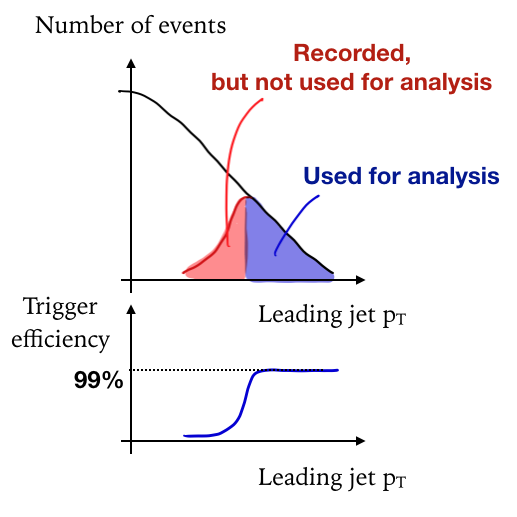
\includegraphics[width=0.5\textwidth]{figures/efficiencySketch}
\caption{\color{black}\label{fig:wastedRate} \small Sketch of how trigger inefficiencies caused by a mismatch between the HLT and offline jet energy scales causes events to be recorded but never used for analysis.} %Trigger operation page
\end{center}
%\vskip-5pt
\end{figure}

Nevertheless, the algorithms used to reconstruct trigger objects must be fast and must not contribute significantly to the overall trigger computing resources, so that only a small fraction of the computing resources is used.
The physics motivation and resource needs will need to be considered in the resource planning of the overall ATLAS physics program.





%% \subsubsection{Reconstruction, calibration and analysis workflow for TLA and TLA+PEB events}

%% \textbf{Reconstruction and calibration} 

%% %Both TLA and TLA+PEB techniques require efficient reconstruction and calibration techniques, since part of the event processing occurs on constrained computing resources.


%% %maybe this is too big picture? but hey, a plot! 
%% %Differences in the energy scale of HLT and offline objects also lead to inefficiencies in the trigger selection, as events that should pass the %% trigger are rejected due to miscalibration in the HLT. 
%% %% As an example, the minimum $p_{\rm{T}}$ threshold applied to jets used in physics analysis is set to be higher than the HLT threshold due to these differences, leading to a substantial waste in terms of events that are recorded but not used for analysis, as shown in Fig.~\ref{fig:wastedRate}. 

%% Additionally, corrections to equalize the energy response across the detector using the balance of forward physics objects to central physics objects could be derived using a quasi-real-time calibration of the data, if calorimeter or LHC conditions were expected to change on a short timescale. 

%% \textbf{Analysis workflow for TLA and TLA+PEB}

%% In order to enable validation of the performance of TLA and TLA+PEB physics objects, it is necessary to retain an event format that includes both regular physics objects and objects presents in the reduced data formats, for a subset of the data.  

%% %edits by Teng Jian Khoo

%% %Q for Lukas/Alison/Gordon: this section is pretty bare but I could add a diagram or write more, what do we want to do here? 

%% %Other things that could be added: 
%% % More of a resource discussion...
%% % Advantages of doing this beyond storage: code optimization, avoiding duplication, reduced waste of data (this is calibration and probably belongs to the analysis section?)
%% % Downsides: need more resources if everyone wants their own PEB so one needs to consider what gets saved carefully depending on the physics case
%% % More details on how one could do reconstruction in partial regions (= learn from trigger)

\subsection{Impact}

%How is the above mentioned R\&D expected to impact physics or costs to the experiment (not sure if this should be here or sprinkled through out this section).
%The activity's impact should be in terms of the "goals" set out in the introduction.
